\section{Results}
\label{sec:results}
\subsection{Reference observations are preserved}
All requested full-vector and active-state comparisons pass at the qualified transaction boundaries. On Linux, the Qwen/Smol deployment compares 6,740 full vocabulary vectors and 4,784 active-state records across geometry, natural requests and terminal cases. Both model families pass all four target-only cut/projection combinations and both speculative paths. Qwen's grouped-query attention has 128-dimensional heads; Smol's multi-head attention has 64-dimensional heads. The qualified arithmetic recipes preserve the reference observations across both structures.

The Llama transfer uses its own family reference. On Vulkan, combined arithmetic and physical-range repair clears the full-vector differences left by arithmetic repair alone, including the 99 committed differences described in Section~\ref{sec:reference}. The 32B mixed-Q4 extension qualifies all six paths and 60 geometry cases. Eight-query qualification additionally checks all requested rows, boundary crossings, rollback, frontier ownership and pending/terminal transitions. Supplement~S1 records the observation counts and boundaries. The clean timing runs then check the corresponding endpoints and execution traces while measuring the qualified implementation.

\subsection{Packing and local cuts contribute at different scales}
\label{sec:factors}
The balanced Qwen experiments cross W/L attention cuts with L4/P projections while fixing the draft policy, input tasks and proposal count. Each of the four speculative paths is measured in the same panel. Figure~\ref{fig:factorial} separates the two component effects.

\begin{figure*}[t]
\centering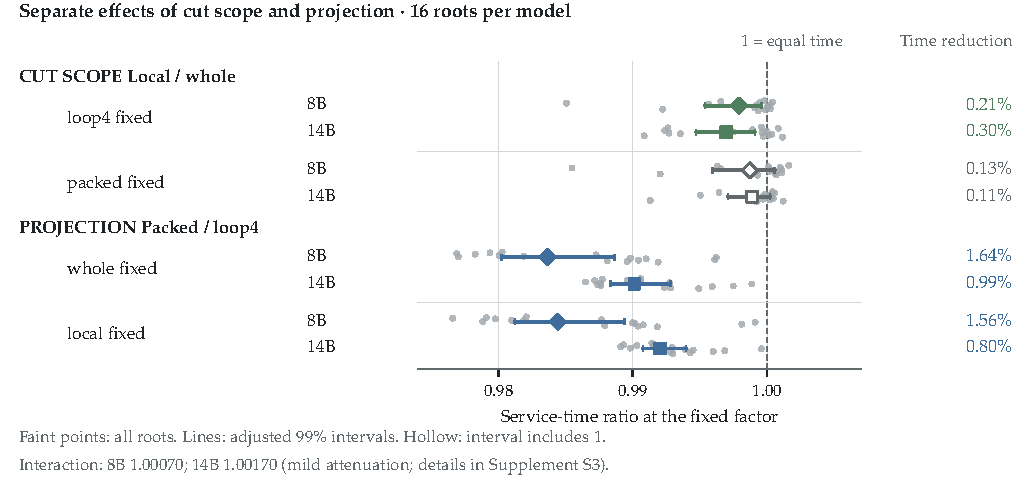
\includegraphics[width=\textwidth]{figures/factorial.pdf}
\caption{Component attribution in balanced A5000 experiments. Points show the 16 task-root ratios; diamonds (8B) and squares (14B) give ratios of total resident-service time. Segments are 99\% paired-root intervals from the five-comparison family. Hollow markers identify intervals that include 1. Projection comparisons fix cut scope; cut comparisons fix projection. The fifth estimand is the interaction in Supplement~S3.}
\label{fig:factorial}
\end{figure*}

Packing reduces service by 1.64\% with whole cuts and 1.56\% with local cuts at 8B, and by 0.99\% and 0.80\% at 14B. The backend-loop4 baseline already moves the loop out of the graph and shares activation quantization, so these differences measure the remaining independent-group packing increment.

Local cuts reduce service by 0.21\% and 0.30\% at fixed loop4 for 8B and 14B. At fixed packing, the reductions are 0.13\% and 0.11\%, with intervals containing 1. The equal-root interactions are 1.000696 and 1.001703, indicating slight attenuation when the components are combined.

\subsubsection{Typed extension to mixed quantization}
For Qwen3-32B, grouping retains the scalar-column Q4\_K and Q6\_K arithmetic and schedules independent columns as channels. Over four roots and four rounds, ordinary grouped execution uses 5.62\% less service with whole cuts and 5.61\% less with local cuts than the graph-level scalar-column loop. All 16 matched pairs improve in each comparison.

A subsequent operator study adds a backend-internal scalar loop: the grouped/backend-loop geometric ratio is 0.8528 over four exposed tensor cells, with mixed paired directions in Q6\_K/q4. Supplement~S3 presents both baselines and all observations. The completed service comparison measures the graph-level grouping implementation; the stronger backend comparison currently supplies operator evidence.

\subsection{Boundary geometry determines the opportunity for local cuts}
\label{sec:geometry}
In the natural 8B factorial, only 20 of 2,224 logical verification cycles require an extra whole-graph boundary split. Local execution uses 2,224 verification graphs; whole execution uses 2,244 for the same target rows. The affected-cycle frequency is 0.899\%. Most verification calls therefore offer no surrounding graph work for local cuts to recover (Fig.~\ref{fig:vulkan}a).

\begin{figure*}[t]
\centering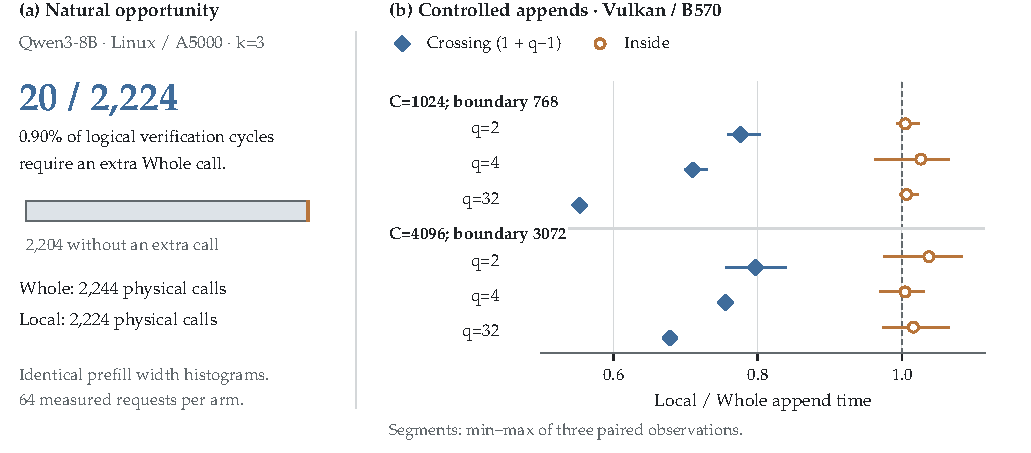
\includegraphics[width=\textwidth]{figures/geometry_opportunity.pdf}
\caption{Where local cuts can help. (a) Natural Qwen3-8B verification on A5000: 20 of 2,224 cycles require an additional whole-graph split, yielding 2,244 whole versus 2,224 local graphs for equal target rows. This is a count of opportunities. (b) Controlled B570 appends at C1024 and C4096: filled markers show boundary crossings and hollow markers their inside controls. Ratios compare local with whole append time; ranges are the minimum and maximum of three paired observations. The two panels measure different quantities.}
\label{fig:vulkan}
\end{figure*}

% Declare the next wide result figure here to avoid a late float.
\begin{figure*}[t]
\centering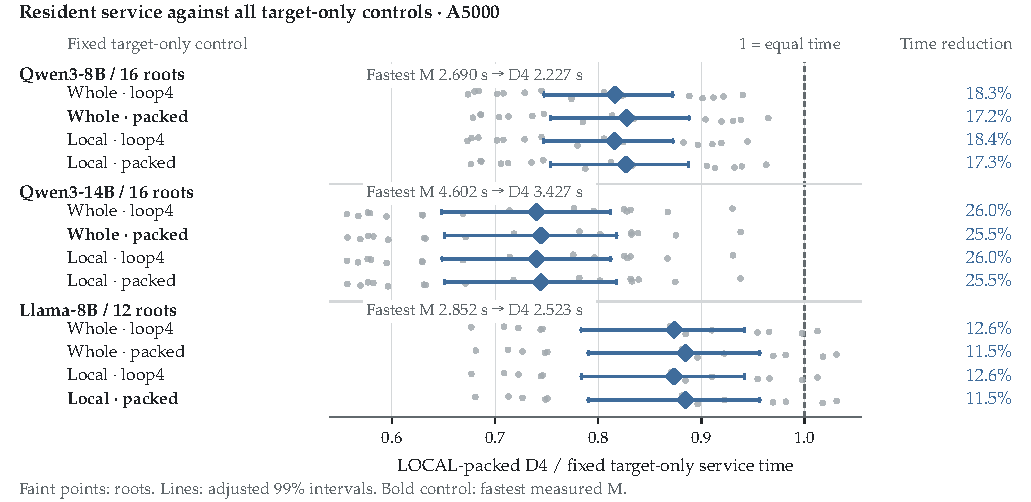
\includegraphics[width=\textwidth]{figures/service_controls.pdf}
\caption{Complete resident-service application comparisons on A5000. Faint points retain all root ratios; diamonds compare LOCAL-packed D4 with each fixed target-only M. Segments are 99\% paired-root intervals from a five-comparison family: the four M comparisons shown here and the W-L4-D4 comparison. Headers give the fastest fixed-M and D4 mean times. Qwen panels share 16 roots; Llama has 12. Table~S1 gives all six arm means.}
\label{fig:service}
\end{figure*}

Controlled Vulkan appends expose the mechanism more directly. We place a call one row before a physical boundary and append $q=2$, 4 or 32 known positions. Whole execution splits the graph as $1+(q-1)$, whereas local execution splits only attention and keeps the surrounding operators wide. Across the six crossing cells at capacities 1024 and 4096, local execution takes 20.34\%--44.68\% less append time. The matched inside controls take approximately 0.43\%--3.74\% more time. Capacity and active-prefix region change together in these cells.

The shape of the split matters. Earlier q32 cells with $16+16$ whole-graph splits included cases favoring whole execution; their complete observations remain in Supplement~S5. Natural-prefix AUTO studies also found little advantage over a whole-graph implementation that rechunks after a boundary. Together, these results explain the two scales in Fig.~\ref{fig:factorial}: local cuts can recover substantial work in a crossing call, while their request-level contribution depends on how often such calls occur.

Packing has a different opportunity. At $k=3$, verification occupies at most four rows and does not enter the wide Q8 packing route. Native execution records locate that route in prefill. Its measured service contribution therefore comes from preserving reference arithmetic while grouping wider known-query work in that phase.

% Declare this wide float early so it stays beside the results it explains.
\begin{figure*}[t]
\centering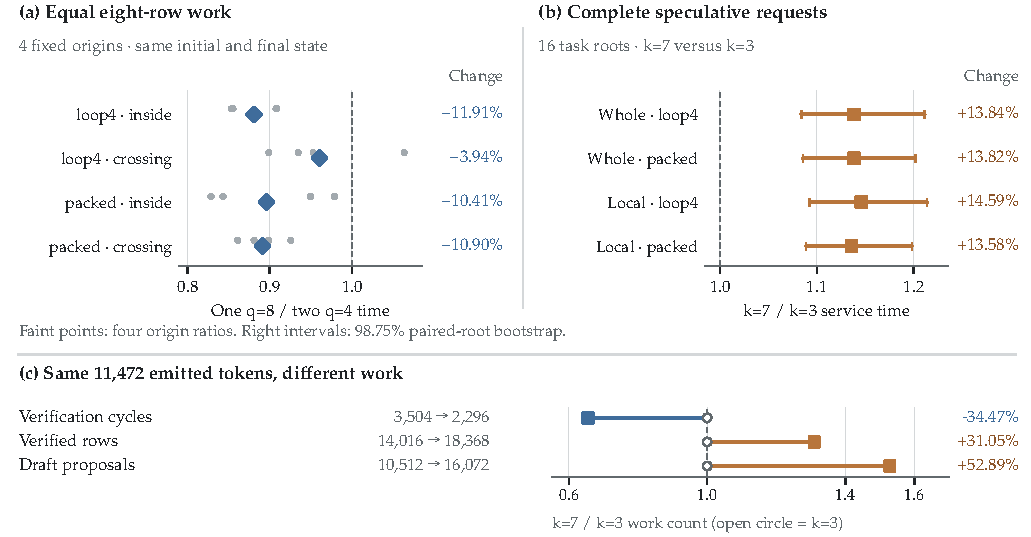
\includegraphics[width=\textwidth]{figures/width_tradeoff.pdf}
\caption{Execution efficiency and live workload. (a) One $q=8$ operation versus two $q=4$ operations from identical state, with the same eight known tokens and all eight requested outputs; faint points retain four development origins. (b) Separate live $k=7$/$k=3$ service comparisons over 16 roots and eight balanced rows, with 98.75\% adjusted intervals. Both widths reserve eight outputs. (c) Work per arm for the same 11,472 emitted tokens: verification cycles fall from 3,504 to 2,296, verified rows rise from 14,016 to 18,368, and draft proposals rise from 10,512 to 16,072.}
\label{fig:width}
\end{figure*}

\subsection{Compatible parallel verification delivers application gains}
\label{sec:application}
Figure~\ref{fig:service} compares complete resident requests with every fixed target-only implementation. LOCAL-packed D4 reduces service relative to all four M controls in each Linux deployment. Against the fastest measured fixed M, mean request time changes from 2.6898 to 2.2269\,s for Qwen3-8B, from 4.6022 to 3.4268\,s for Qwen3-14B, and from 2.8515 to 2.5230\,s for Llama-8B: reductions of 17.21\%, 25.54\% and 11.52\%. The adjusted intervals support each fixed-M comparison.



These gains are the value of the complete speculative application using reference-compatible target execution. Whole-graph execution also supports that application. The independent contributions of packing and cut placement are the smaller effects measured in Section~\ref{sec:factors}.

The 14B improvement persists beyond the resident timer. Its measured-request burst takes 294.632\,s for the fastest fixed M and 219.405\,s for LOCAL-packed D4. Including model loading, integrity checks, primers and the requests, native-worker time falls from 662.546 to 594.559\,s, a 10.26\% reduction. Llama's resident requests improve, but its short worker workload favors M after initialization is included. The Windows Qwen3-8B study separately reports 29.11\% less resident time and 26.00\% less worker time; the Linux Qwen studies reuse the Windows task records with separate references and measurements. Supplement~S2 gives the complete costs.

On the 32B mixed-Q4 panel, ordinary grouped generation is fastest; grouped D4 takes 14.00\% more resident time. In the B570 resident pilot, local verification halves the occupied target-graph count relative to the earlier scalar speculative path, but draft work leaves the complete speculative request slower than ordinary generation.

\subsection{Wider execution and the cost of live work}
\label{sec:width}
The eight-query implementation retains the reference arithmetic and supports $k=7$ proposals plus the pending position. We evaluate physical execution width and live proposal width with separate comparisons (Fig.~\ref{fig:width}).



On the Windows RTX, one q8 call uses 3.94\%--11.91\% less aggregate operation time than two q4 calls across the four fixed method/geometry cells. A matched-history A5000 diagnostic on one exposed origin reports q8/q4-pair geometric ratios of 0.9904 and 0.9781 for loop4, and 0.9370 and 0.9476 for packing. Each A5000 cell has four process clusters; loop4 includes mixed process-level directions. Supplement~S4 retains these observations and the separate live pilot.

In live generation, however, k7 changes the work. Per arm, verification cycles fall from 3,504 to 2,296, while verified rows rise from 14,016 to 18,368 for the same 11,472 emitted tokens. Acceptance among inspected proposals changes little, from 87.47\% to 87.93\%, but accepted proposals as a fraction of all proposals fall from 75.42\% to 56.94\%. Longer proposals spend more work on suffixes that are not consumed.

Consequently, k7 takes 13.58\%--14.59\% more complete service time than k3 across the four methods. For LOCAL-packed, the additional 24.897\,s over 128 requests consists chiefly of 13.567\,s more verification and 13.224\,s more draft proposal, offset by 2.792\,s less draft synchronization. Output copying adds 0.252\,s; the remaining phases close the balance.

The disjoint phase account is
\begin{equation}
 T_{\mathrm{spec}}=T_{\mathrm{target}}+T_{\mathrm{draft}}+T_{\mathrm{state/output/host}}.
 \label{eq:cost}
\end{equation}
The equal-work panels show lower aggregate cost for wider execution. In live generation, the additional target and draft rows outweigh that saving, leaving k3 with the lower complete cost.
